\section{System Overview}

Motivated by outliers problem, we named our system for Nearly No Outliers (N2O) expressed our best wishes and indicated N2O’s mission. As far as we know, the other N2O system in the world is primarily concerned with introducing fuel and nitrous into the engine's cylinders, and combining them for more efficient combustion. It is typically used to provide an instantaneously speedup for auto, while our N2O system can provide a persistently speedup for job schedulers commonly used in cluster.

N2O contains two main components, the instrumenter and speculator. The instrumenter has a perfect partner, the sampler, which collects sampling data about code coverage of a variety of executions. Though the instrumenter can finish the instrument task for tracing progress itself, an additional overhead as much as several percentages of execution time is unavoidable. This is unacceptable in production system, but with the sampler‘s cooperation, overheads can be cut down, even negligible. Details will be shown in the evaluation part. N2O also provides a flexible job description template for wrapping stand-alone binary to a customized job that can be submitted to a job scheduler and speeded up by N2O.

\begin{figure}
\centering
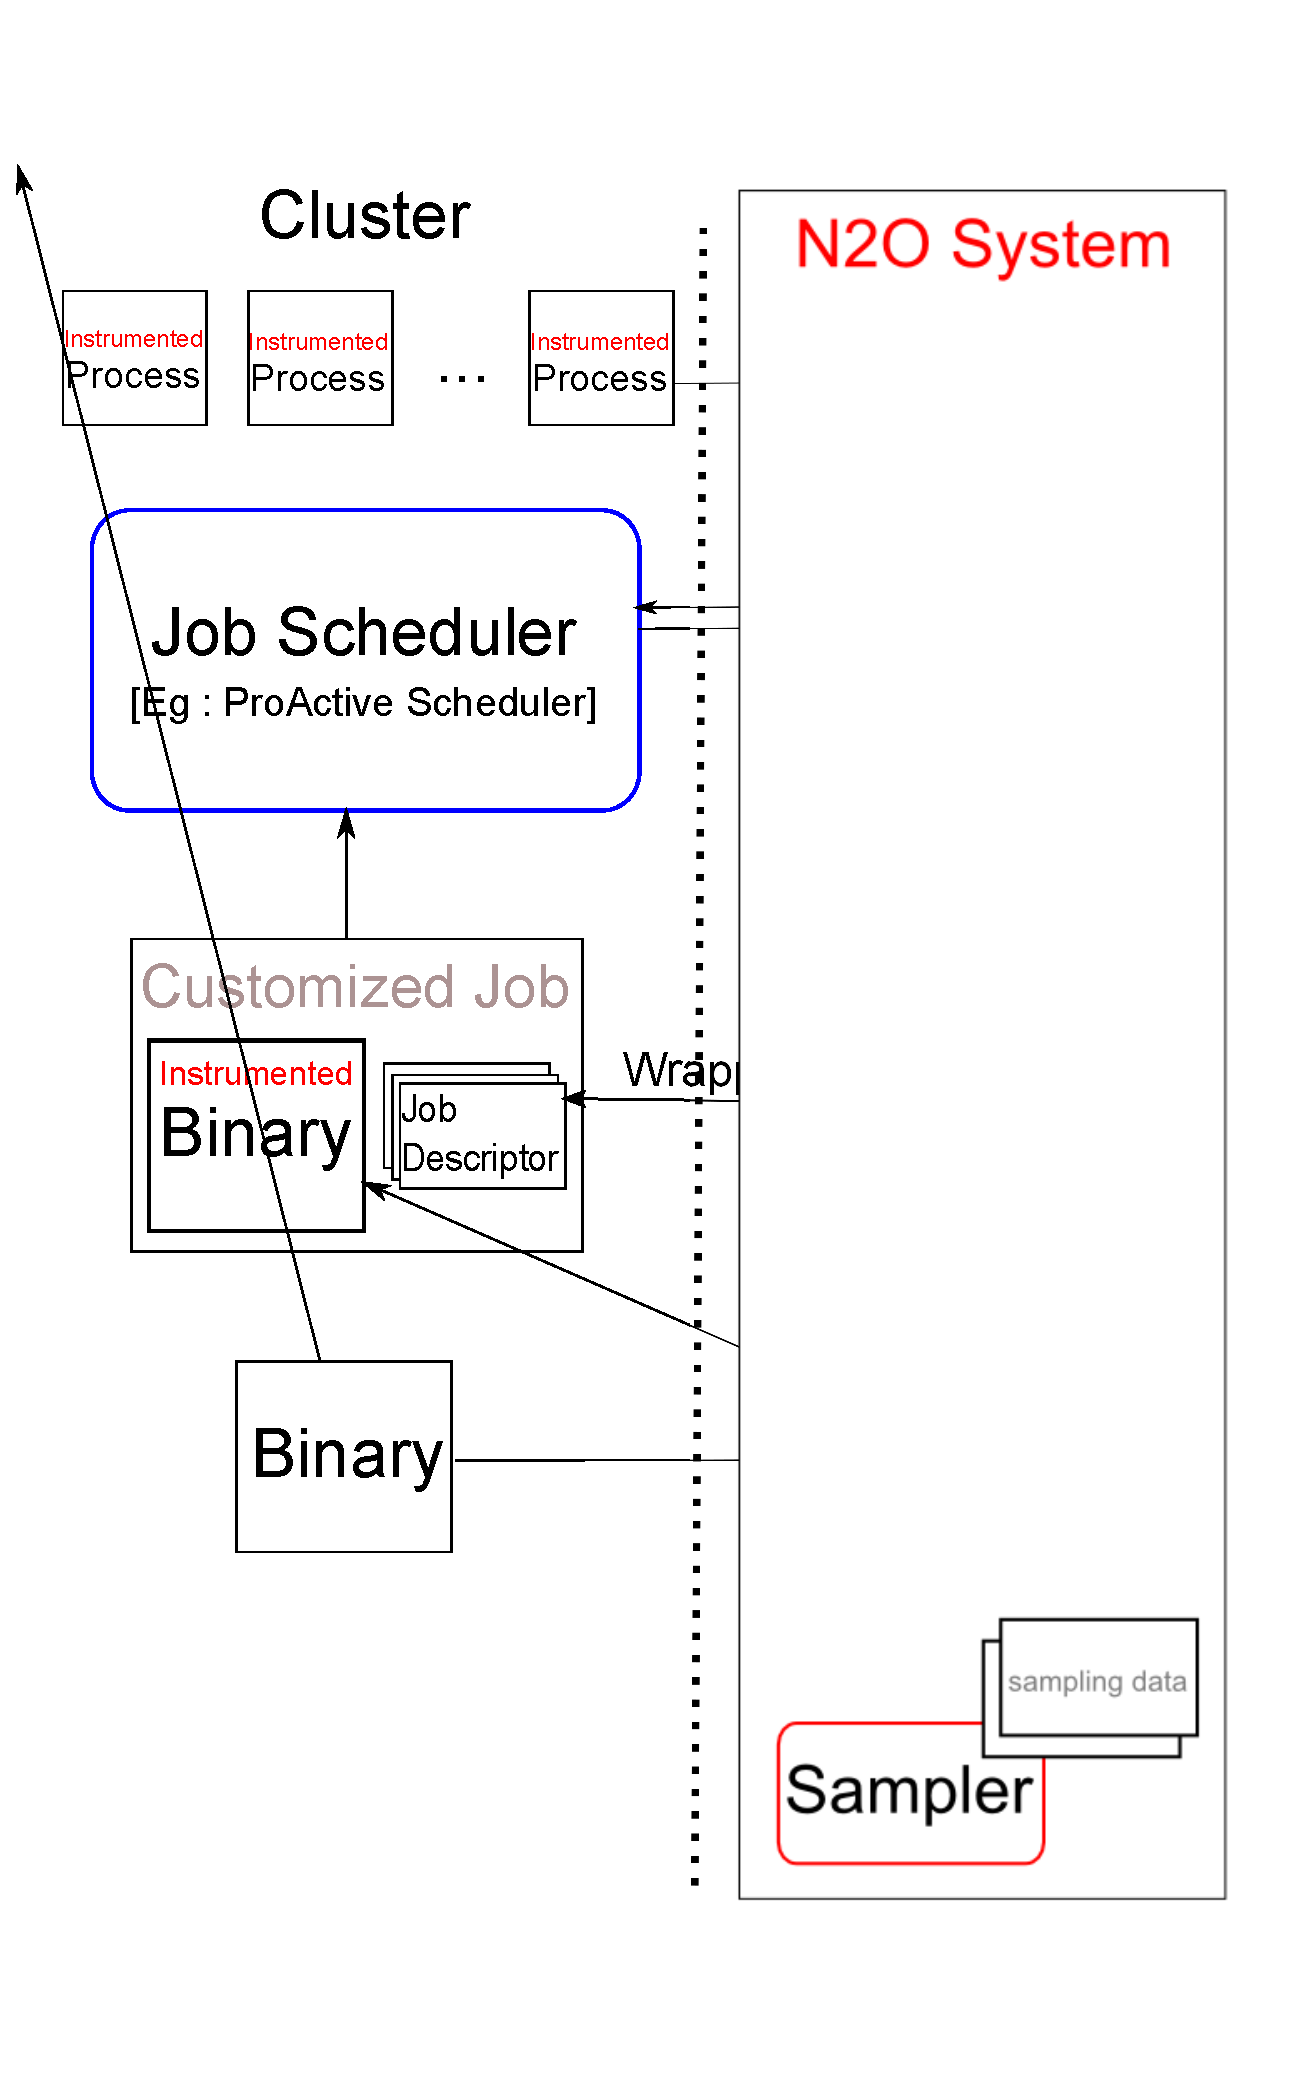
\includegraphics[width=0.9\columnwidth]{figures/N2O_arch.eps}
\caption{N2O Architecture}
\label{figure:n2oarch}
\end{figure}

We carefully designed N2O to make sure of its independence with job scheduler which benefits users adapting to different job scheduler easily. As Figure 1 shown, the only interactive between N2O and job scheduler is the interface for obtaining job status information and request to kill and start a job or task. These abilities can be easily satisfied by any scheduler control interface, such as control script provided by ProActive Scheduler or command line tools provided by Condor.

The job description template we provide can be used immediately in ProActive Scheduler, because of following ProActive Scheduler’s job description XML structured rules. But it doesn't mean something dependence, It’s easily to change to another scheduler with tiny modification on format. And except for XML descriptor, there are three extra shell scripts for splitting, wrapping native task and merging the results if needed. The shell scripts will be submitted and executed as normal tasks on job scheduler.

Taking a picture rendering job for example, there may be three phases for this job: 1. splitting the image into small pieces, 2. rendering them in parallel, 3. merging the rendered parts. These three phases exactly match N2O‘s three shell script templates: split script, operation script and merge script. Users just need to add an image cutting command into the split script, which may be optional for other jobs and modify the default procedure copy input files to the destinations as needed. In the operation script, the native task must be  expressed as a command, a daemon process for trace log transferring is also launched default. When all parts of result has been collected, a merge image command added in the merge script, optional for other jobs too. As described above,  users have an extreme flexibility to make their native tasks massive parallel. On the other hand it means N2O do not provided any file transfer or data placement service and so on, which have been provided by job schedulers or a distributed file system of cluster itself.

In the next sections, we will mainly illustrate the design and implementation of binary instrumentation and speculative execution in N2O system. 